Dado un grafo no dirigido $G$ con $n$ nodos y $m$ aristas. Queremos encontrar en él todas las componentes conexas, es decir, varios grupos de vértices tales que dentro de un grupo se puede llegar a cada vértice desde otro y no existe camino entre diferentes grupos. Por ejemplo en la imagen de abajo tenemos un grafo con tres componentes conexas.

% TODO: \usepackage{graphicx} required
\begin{figure}[h!]
	\centering
	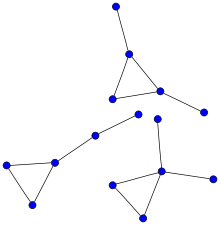
\includegraphics[width=0.25\linewidth]{img/220px-Chromatically_equivalent_graphs.svg}
	\label{fig:220px-chromaticallyequivalentgraphs}
\end{figure}
